\section{Experimental Evaluation}
\label{sec:results}

\subsection{Experimental Setup}

As described in Section \ref{sec:system}, all results were collected on the physical dual-SO-101 setup. The tray carried a glass filled with water, resting on the tray center. Each trial began with the arms near \texttt{HOME} and the tray placed in a varied, but central position within the recorded workspace.

\subsection{End-to-End Success Rate \& Failure Modes}

A set of 50 trials were run using our algorithm, during which the failures at each phase were noted. Figure \ref{fig:failure rate per phase} illustrates the total failures per phase out of total number of trials that made it to that phase. Out of the 50 trails, the arms made it back to the \texttt{HOME} position successfully 37 times, which is a 74\% success rate. A clear pattern was established where failures concentrate at the start of the trajectory when the arms must locate and attach to the tray, vanish through the middle of the lift and translate, and return briefly during \texttt{LOWER}. 

\begin{figure} [H]
    \centering
    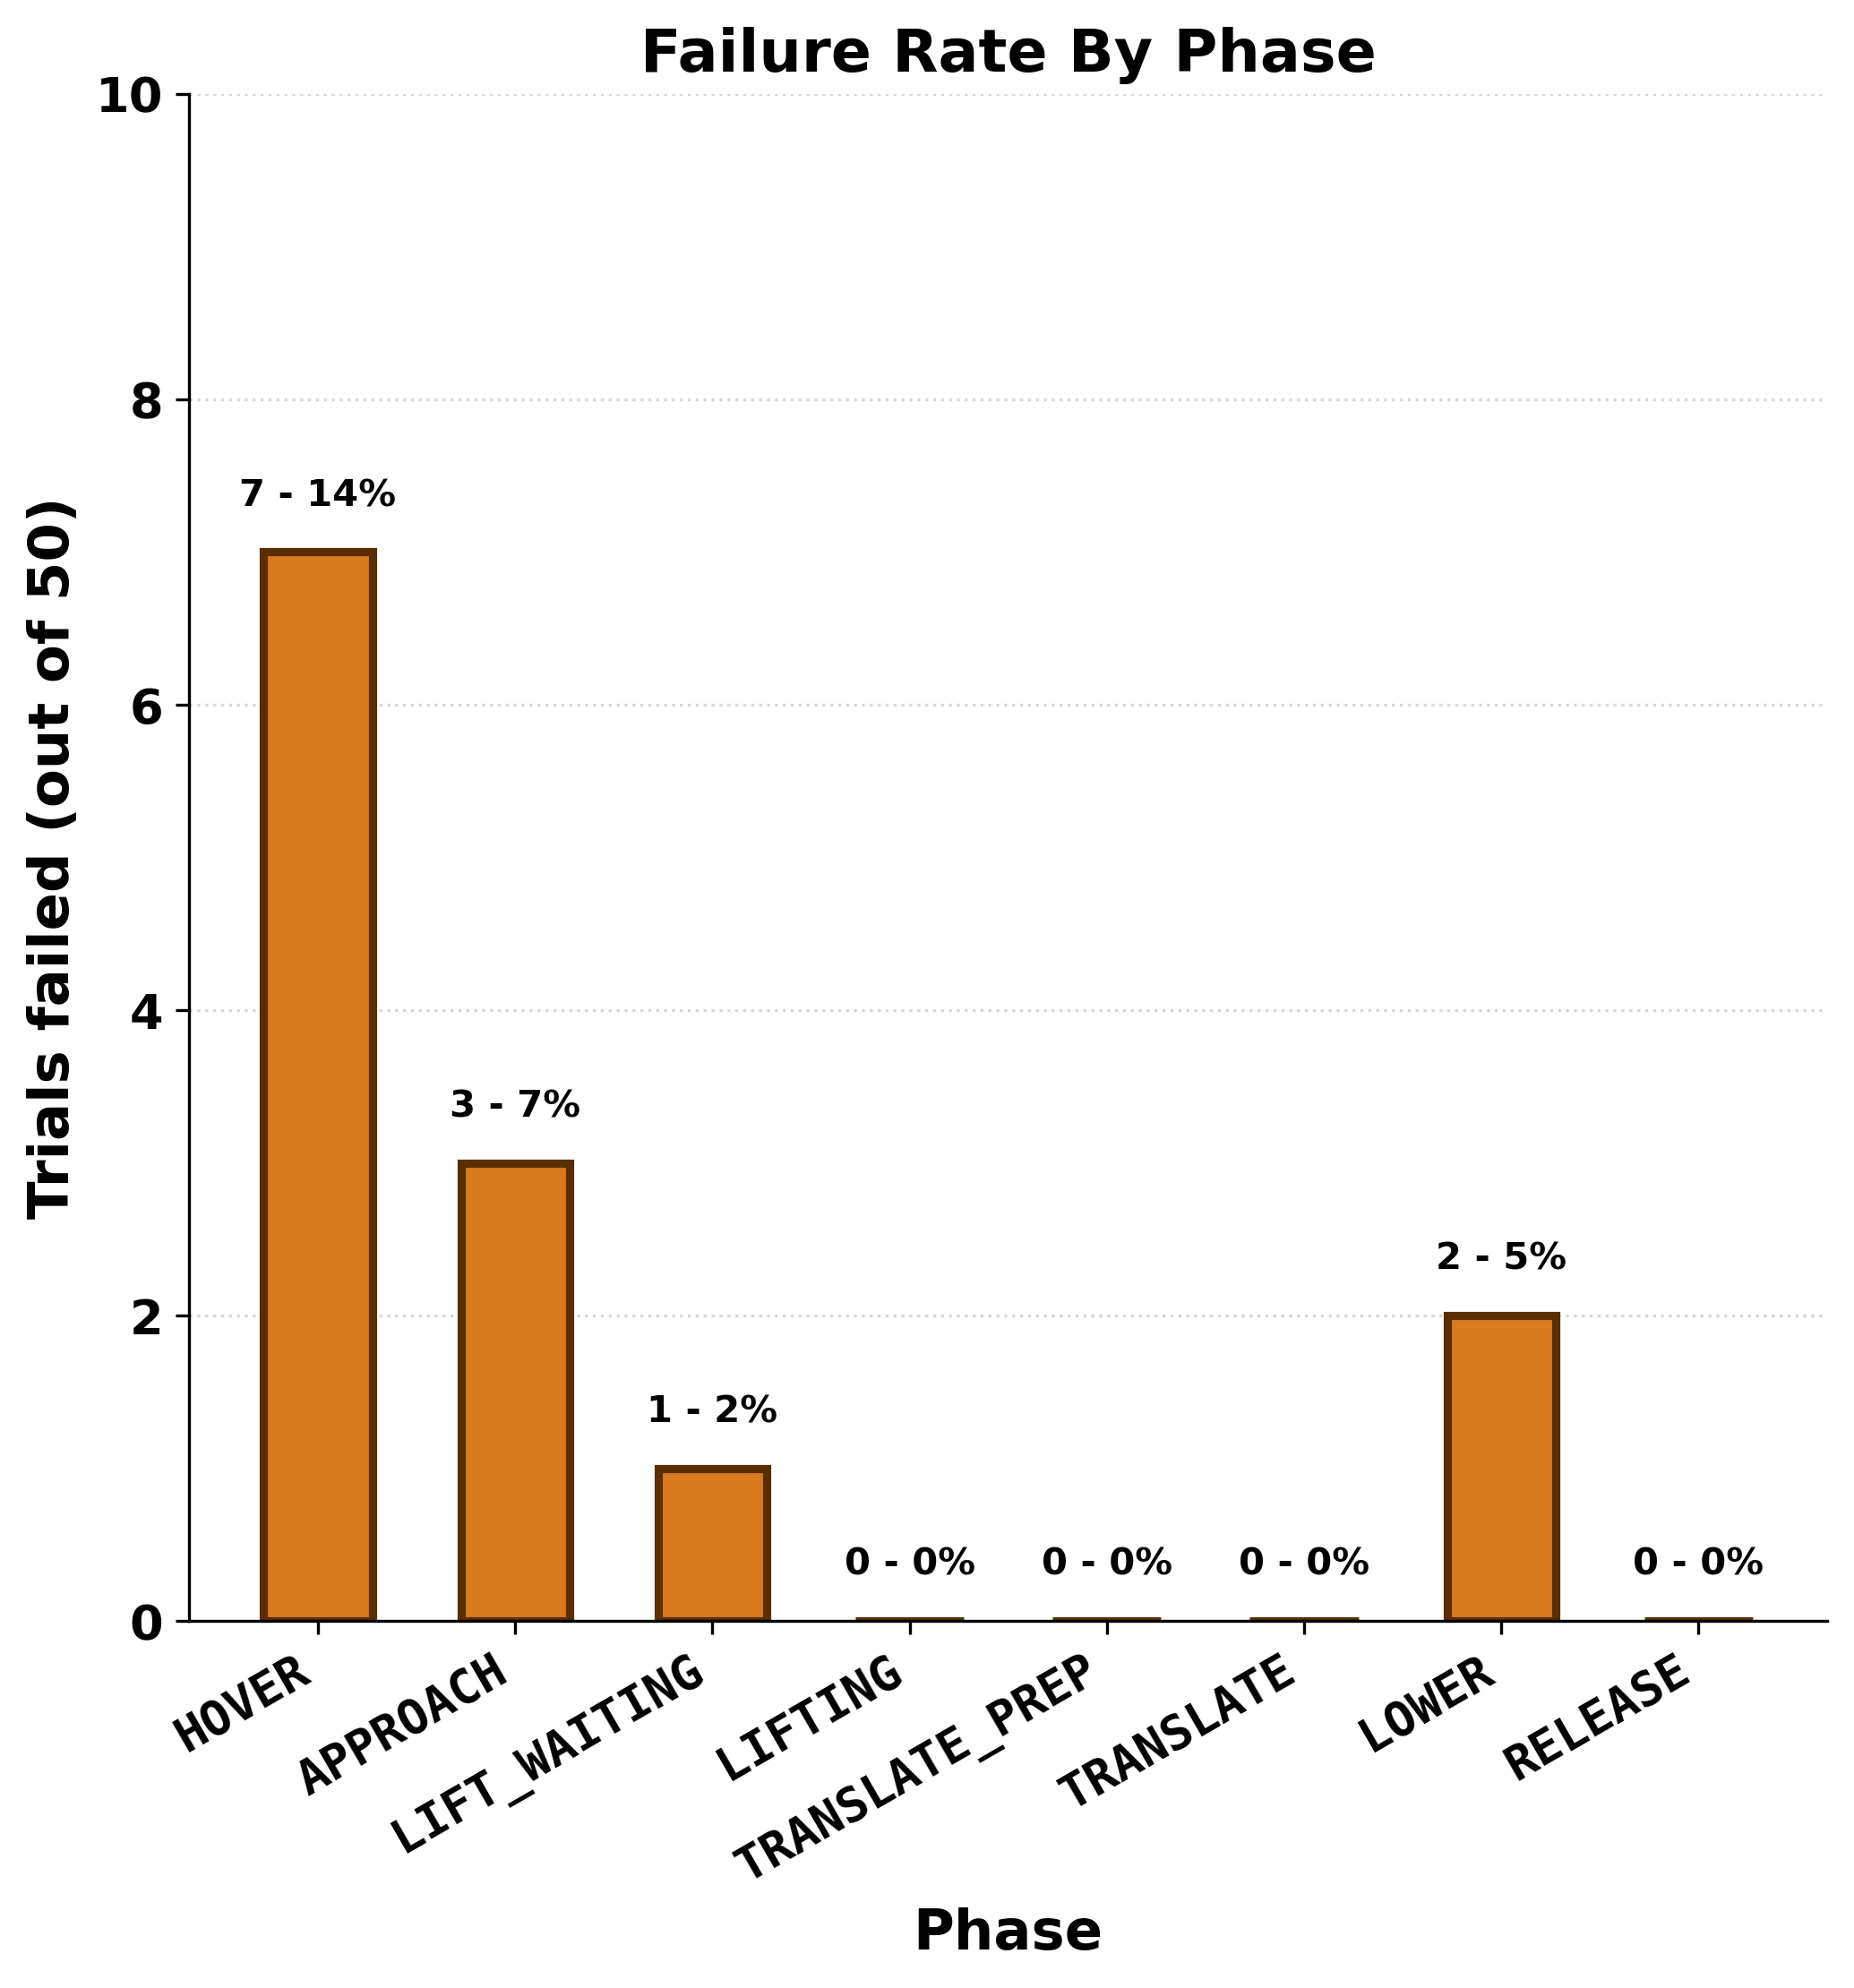
\includegraphics[width=1\linewidth]{subtex//images/failure_rate_by_phase.png}
    \caption{Failures and failure rates during 50 trials. Percentages represent failure rate relative to the total number of trials that made it to that phase.}
    \label{fig:failure rate per phase}
\end{figure}


The failure modes for each phase are described below. 
\newline

\textbf{\texttt{HOVER} (7\,/\,50, 14\%).} \texttt{HOVER} is the most failure-prone phase, with two distinct failure modes. In the more common mode, the arm converges to a position slightly offset from the actual tray marker. This is close enough that the convergence test passes, but offset enough that on APPROACH the gripper hits the tray. This failure traces directly to \texttt{POSITION\_OFFSET} (Section \ref{sec:hover}), which was the only parameter in the entire pipeline that required precise per-arm tuning very often. The second failure mode is a non-convergence where the planar error never falls below \texttt{CONVERGENCE\_THRESHOLD\_M} for three consecutive frames, and the arm stalls in HOVER indefinitely. Loosening the threshold trades one mode for the other.

\textbf{\texttt{APPROACH} (3\,/\,43, 7\%).} \texttt{APPROACH} has no closed-loop correction during descent as it just steps straight down from wherever \texttt{HOVER} ended with a descent delta. These pre-alignment problems are considered \texttt{HOVER} failures, but have the potential to be remedied by this phase. When the gripper was aligned, however, and the descent caused a misalignment, or the arm did not descend the right amount, an \texttt{APPROACH} failure was recorded. A potential future fix is to implement visual servoing during the descent rather than cutting to a fixed delta, which would help this phase as well as the previous, but requires inverse kinematics outside the motion map plane.

\textbf{\texttt{LIFT\_WAITING} (1\,/\,40, 2.5\%).} A single trial failed when one arm's nudge produced a tray-marker rise below \texttt{TAG\_RISE\_THRESHOLD\_M} $= 3$\,mm. The handshake is designed to refuse false positives, so the listening arm waited indefinitely and the system just stopped. Lowering the threshold would have caught this trial but would also raise the chance of false positive triggering due to measurement jitter. Increasing the nudge-lift magnitude would also fix this problem, but increases the risk of tilting the tray too much and causing the glass to move or spill.

\textbf{\texttt{LOWER} (2\,/\,39, 5\%).} Both \texttt{LOWER} failures were due to the same failure mode. One arm reached the end of its lowering trajectory while still seeing itself as the lower side by more than \texttt{TILT\_PAUSE\_THRESHOLD\_M} $= 5$\,mm, so the tilt-pause rule of \cref{algo:lower} held it indefinitely and the gripper never released. To fix this, more accurate lowering waypoints during data collection around the table contact height would close this gap. It was never the case that the arms released before the tray had reached the table, so a slightly higher waypoint would be beneficial.

\textbf{Phases with zero failures.} \texttt{LIFTING}, \texttt{TRANSLATE\_PREP}, \texttt{TRANSLATE}, and \texttt{RELEASE} produced no failures across all trials that reached them. The successful synchronized lift is attributable to \cref{algo:lift}'s self-throttling rule. The translate phases benefited from the TPU gripper tips, whose flexibility absorbed small marker jitter and pose mismatches that would otherwise have caused tray slippage. The hardcoded phases at the beginning and end also never failed since those were done as a simple interpolation between two points.



\subsection{Coordination Metrics}

\begin{figure} 
  \centering
  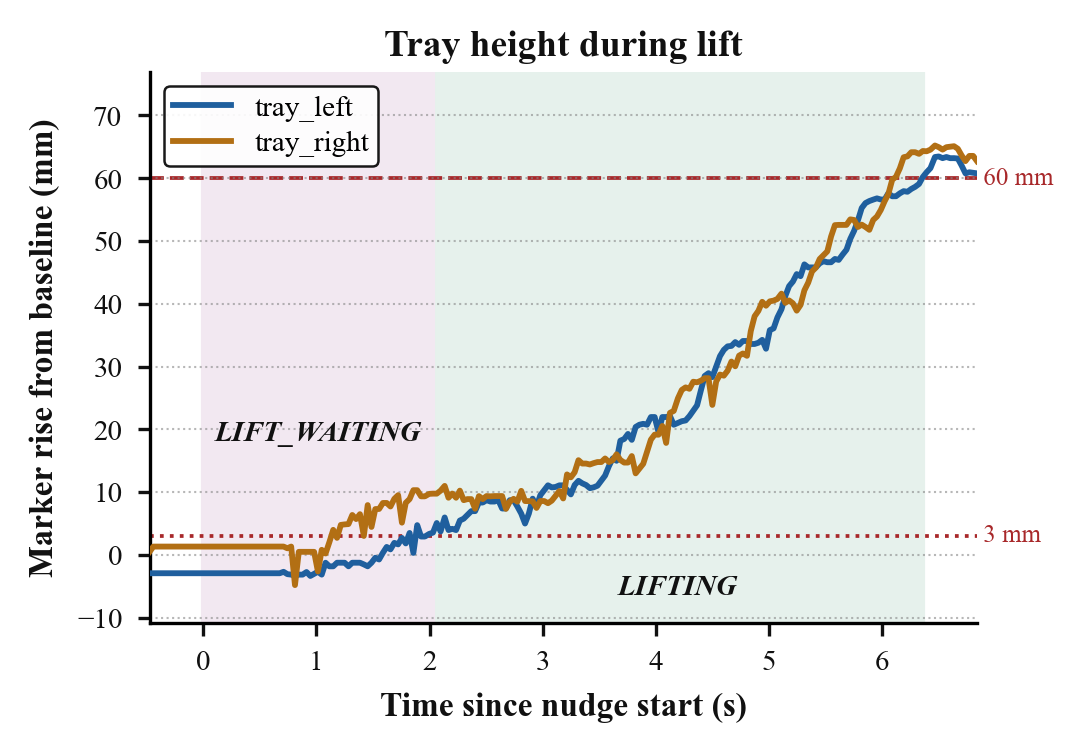
\includegraphics[width=1\columnwidth]{subtex/images/lift_height.png}
  \caption{Synchronized ascent produced by the self-throttling rule
  of \cref{algo:lift}. Each arm only commands an upward step when
  its own side is at or below the other side.}
  \label{fig:lift}
\end{figure}

\begin{figure}
\centering
  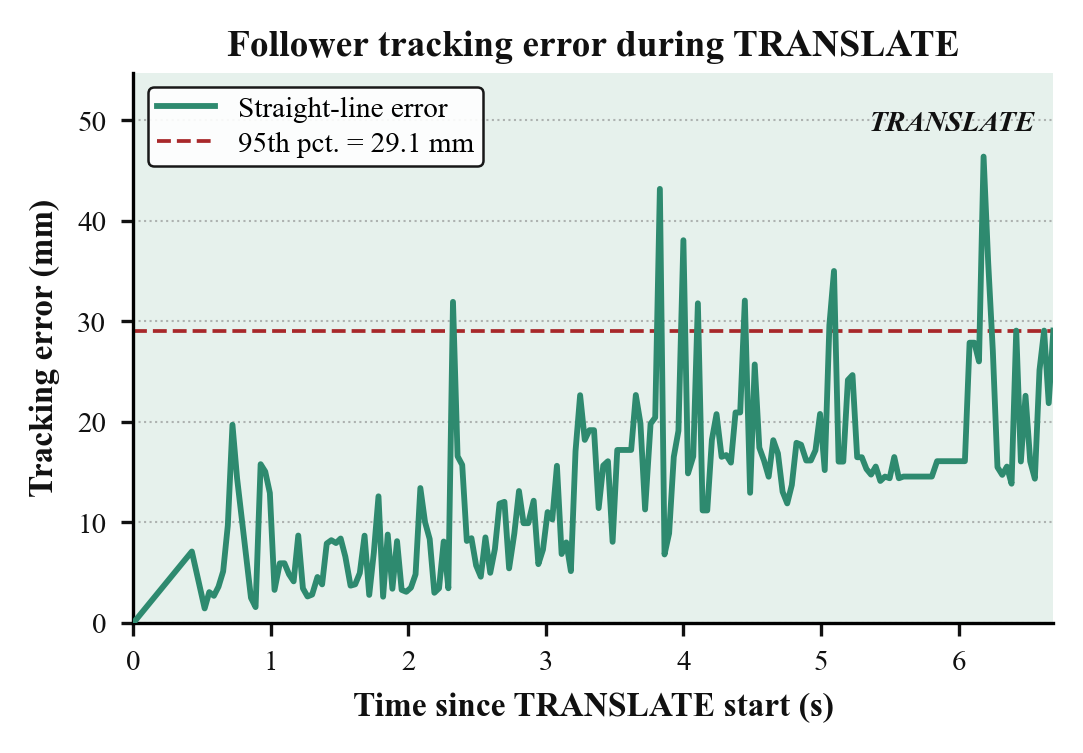
\includegraphics[width=1\columnwidth]{subtex/images/translate_follower_error_ep004.png}
  \caption{Follower tracking error during \texttt{TRANSLATE} for a
  representative trial. Defined as
  $\Vert\,\vec{x}_{\text{grip},R}(t) - (\vec{x}_{\text{grip},L}(t) +
  \vec{o})\,\Vert$. The follower starts close to the desired position, but drifts further from the goal position as the leader moves away.
  The strong EMA on the follower's
  target ($\alpha_f{=}0.1$, \cref{algo:translate}) intentionally
  trades latency for rejection of the very high measurement noise.}
  \label{fig:translate-error}
\end{figure}




% these directly should reference the graophs
A simple pass or fail does not capture how cleanly the coordination ran on a successful trial. Two quantitative signals were tracked in order to best characterize the quality of the coordination:
\begin{itemize}
  \item \textbf{Tray heights.} The maximum $|y_{\text{tray},l}-
        y_{\text{tray},r}|$, or tray-marker height disagreement, observed during \texttt{LIFTING}. This measures how well \cref{algo:lift}'s self-throttling rule keeps the tray level and is shown in \cref{fig:lift}. A desynchronized nudge-lift is evident in the graph, followed by a flat region for the right arm as it waits and watches for the left arm's lift. Once both arms transition to lifting, they form this beautiful reciprocating pattern in which each arm becomes the higher one, then waits. The maximum tray tilt during this trial is approximately one centimeter, which corresponds to a maximum tray angle of 4$^\circ$ given the 14 cm marker spacing. This is much less than the tilt required to cause movement of the glass.
  \item \textbf{Translation follow error.} Shown in \cref{fig:translate-error}, this is the 3D base-frame distance from the right grip target
        ($\vec{x}_g^\text{\,left}+\vec{o}$) to the right gripper's actual position during \texttt{TRANSLATE}, with the follower tracking the leader's gripper per Algorithm \eqref{eq:offset}. The motion during each trial is quite smooth so evidently there is very high measurement noise from one or both markers. This success is attributed to the mechanical design and material improvements of the end effector assembly, as well as the EMA during control.  
\end{itemize}

